\begin{enumerate}[label=\thesection.\arabic*.,ref=\thesection.\theenumi]
\numberwithin{equation}{enumi}
\item
Sketch direct and inverse polar plots for a unity feedback system with open loop transfer function
\begin{align}
G(s) = \frac{1}{s(1+s)^2}
\end{align}
 
\\
\solution  
For Unity feedback system, the closed loop transfer function
\begin{align}
\frac{Y(s)}{X(s)} = \frac{G(s)}{1+G(s)}
\end{align}
Therefore;
\begin{align}
\frac{Y(s)}{X(s)} = \frac{\frac{1}{s(1+s)^2}}{1+\frac{1}{s(1+s)^2}}
\end{align}
which gives;
\begin{align}
\frac{Y(s)}{X(s)} = 
\label{eq:sec_order_op}
\end{align}
%
The following code plots $c(t)$ in Fig. \ref{fig:sec_order}
\begin{lstlisting}
codes/ee18btech11002/plot.py
\end{lstlisting}
\begin{figure}
\centering
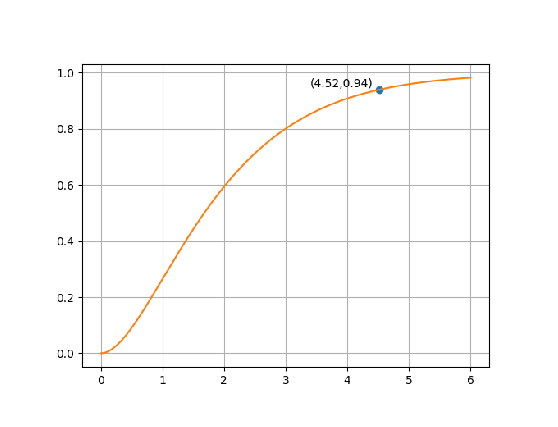
\includegraphics[width=\columnwidth]{./figs/ee18btech11002.eps}
\caption{}
\label{fig:sec_order}
\end{figure}
\item Find the steady state response of the system using the final value theorem.  Verify using 
\ref{eq:sec_order_op}
\\
\solution 
To know the steady response value of c(t), Using Final value theorem:
\begin{align}
\lim_{t\to\infty} c(t) = \lim_{s\to 0} sC(s) 
\end{align}
We get
\begin{align}
\lim_{s\to 0} s \brak{\frac{1}{s}}\brak{\frac{1}{1+2s+s^2}} = \frac{1}{1+0+0} = 1
\end{align}
To verify, calculate
\begin{align}
\lim_{t\to\infty} c(t) = (1-0-0) = 1 
\end{align}
\item Find the time taken for the system output c(t) to reach 94\% of its steady state value.
\\
\solution 
Now, 94\% of 1 is 0.94, so we should now solve for a positive t such that
\begin{align}
1 - e^{-t} - te^{-t} = 0.94
\end{align}
The following code 
%
\begin{lstlisting}
codes/ee18btech11002/solution.py
\end{lstlisting}
%\lstinputlisting{./}
provides the necessary solution as 
%the attached code gives us the solution for the equation
%and t turns out to be
\begin{align}
 t = 4.5228
\end{align}

\end{enumerate}
